\chapter{Detail Arsitektur Sistem}
\label{appendix:detailed-architecture}

Gambar \ref{fig:detailed-architecture} menunjukkan gambaran detail arsitektur sistem eksperimen yang digunakan dalam penelitian ini. Arsitektur ini mencakup komponen-komponen utama yang berperan dalam pengumpulan data, pengelolaan konsistensi, dan replikasi data antar \textit{Node} seperti yang telah dijelaskan pada Bagian \ref{sec:rancangan}

\begin{figure}[ht]
	\centering
	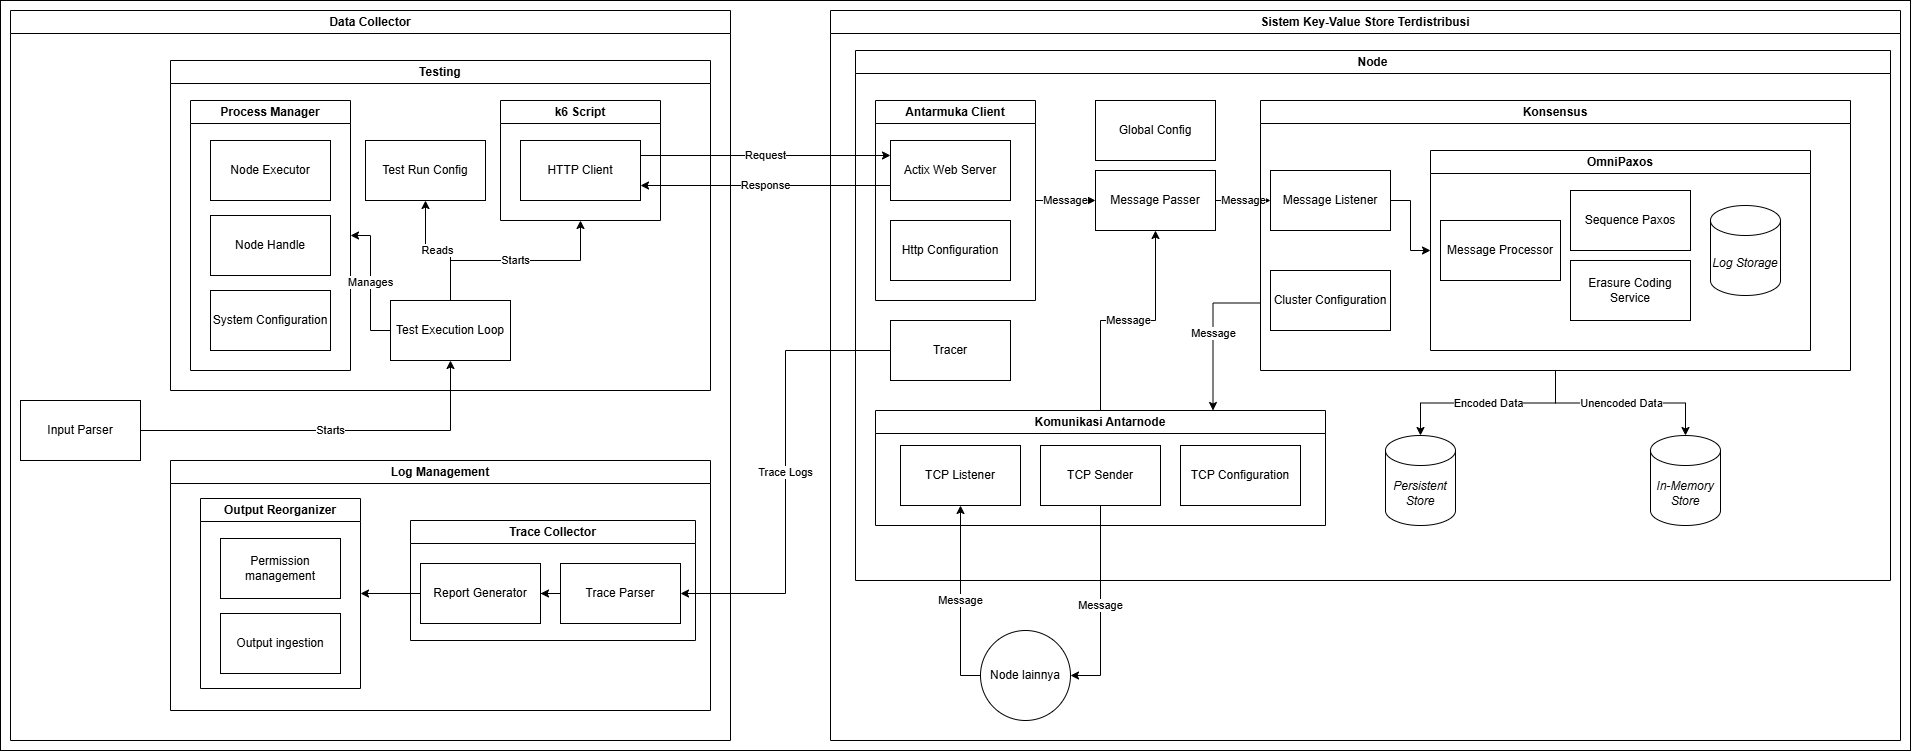
\includegraphics[width=\textwidth]{resources/appendix/detailed-architecture.png}

	\caption{Gambaran Detail Arsitektur Sistem Eksperimen}
	\label{fig:detailed-architecture}
\end{figure}